% !TEX root = ../Thesis.tex
% !TEX spellcheck = en-US

\chapter{GNS3}
\label{ch:gns3}

% GNS3, whose original name was ``Graphical Network Simulator-3,'' is a software project, comprising several distinct components and, despite the ``simulator'' in its name, it falls under the category of emulators (cf.~\ref{sec:emulationsimulation}): its operation runs real code accross all the layers of the stack. % TODO try to (either with a source, or speculating) relate the name with ns-3
% TODO also: cite the source for the name
% By ``as a whole,'' it is meant that, as shall be seen later, although some of its components, like the Dynamips program, are emulators in a very strict sense---i.e. its purpose is to run real machine code on a different hardware architecture (than its native one)---, it differentiates itself, on a high-level perspective, from a simulator which is a program designed to execute a mathematical model, processing modeled events as internal data-structures with a collection of preset algorithms that somehow mimic (a part of) the reality. % TODO: delete?

% Note that a necessary step towards the goal of this this thesis is to systematize a technical description of the architecture and functional underpinnings of the GNS3 system.
% How does it interact with the hardware and software it is running in, how much resources does it take to work with GNS3 according to the ``mode'' it is running in, etc., as that is an aspect that is yet to be further explored for, at least, the following reasons:  % TODO improve the writing how is etc written in Engilsh?
% on the one hand, the consulted academic material (i.e. research papers, mostly) is very brief and omissive in regards to the design, architecture and implementation of GNS3, and so is the official website and documentation; on the other hand, many interesting details are in the ``paraofficial'' videos available via YouTube, mostly by David Bombal\footnote{\url{https://www.youtube.com/channel/UCP7WmQ_U4GB3K51Od9QvM0w}}, namely a comprehensive overview of the architecture (compared with the functionality) of GNS3 by its creator, Jeremy Grossmann, and essentially are not anywhere else, at least from authoritative sources. % TODO same as the previous "sentence". Cite the videos (how and which ones?)

% TODO add a figure (a screen shot) showing the "official" submitter of GNS3 videos (and maybe the channel and/or links from the gns3 official website)

% end of intro

% The first section of this chapter explains the motivation behind the creation of GNS3, as that fact determines implementation and functional aspects of this piece of software.
This chapter consists in a detailed analysis and study of one of the two examples given in chapter~\ref{ch:examplesofemulators} which were chosen to be looked into more depth and, later, compared against each other---the GNS3 emulator.
First, two sections present GNS3 from a more technical angle:
  \begin{enumerate*}[label=(\roman*), itemjoin={{, }}, itemjoin*={{, and }}]
  \item a description of the architecture and the main design characteristics of GNS3 are explained, giving a good overview of the kind of setup it needs, and in what kind of environments it can be executed and inherent scalability features
  \item the implementation solutions chosen by GNS3's developers to provide its high-level functionality.
  \end{enumerate*}
Then, the chapter finishes by presenting a case-study that directly addresses the problem which motivates this thesis and describes how GNS3 offers solutions for that problem, and then performance and resource consumption considerations, result of the observation done mainly during the performance of the case-study, are exposed in a systematic way.

% Section "GNS3's purpose and raison d'être"
% \section{GNS3's purpose and \emph{raison d'être}}
\label{sec:gns3why}

The GNS3 project was co-created by Jeremy Grossmann as a University project, at the Ecole informatique Epitech, part of the \emph{EPITECH Innovative Project (EIP)}\footnote{\url{https://eip.epitech.eu/2013/gns3/en/index.html}, accessed on December 2019}.
There is also a blog\footnote{\url{http://gns3.blogspot.com/2007/}, accessed on December 2019}, whose first posts date back to 2007, that announces the first ``beta'' releases of the software and gives the details about the inception of GNS3, and also lists the original developers of the project.

It may be speculated that GNS3's first ``appeal'' was supplying students of Cisco certifications with a self-study tool more powerful that anything before, one that allows for the creation of arbitrary network topologies and practice their skills with the same software stack that is used in real Cisco devices and the hosts connected to them---from the operating system, up until application--level network utilities---, without having to use the expensive official solutions for that purpose, or depending on a real, physical networking laboratory.
However, despite having kept a strong relation with training for Cisco CCNA and related certifications~\cite{thebookofgns3,gns3netsimguide}, the magnitude of the project, part of which comes from an inherent extensibility, has made it suitable for a myriad of use-cases.

In the industry, GNS3 naturally can come handy as a tool to prototype and test a topology for a real organization network, in the context of the practice of a network professional.
But also, in the age of the DevOps philosophy---a set of practices and methodologies/philosophies for faster delivery of applications and services---, of which \emph{infrastructure as code} is one of the culprits~\cite{awswhatisdevops}, it can be of value for software engineers to test distributed applications that depend on certain network behaviors.

% At the moment of the writing of this thesis, version 2.2 has recently came out\footnote{\url{https://github.com/GNS3/gns3-gui/releases/tag/v2.2.0}}.
% This version brings a lot of improvements and new features, like the new web UI or ``physical'' link state detection for QEMU nodes~\cite{releasenotesgns3v22}, and at the same time some of the ways GNS3 has been typically used are changing---such is the case of the discouragement of the usage of Dynamips and VPCS (in detriment of virtualized versions of IOS or others, or Docker containers for ``emulating'' hosts, respectively)~\cite{ytdynamipsvpcs}.


% Section "General architecture"
\section{Architecture and building blocks}
\label{sec:gns3architecture}

A good written, comprehensive description of the GNS3 architecture and technical details is lacking.
There is a page, on the online developers-oriented documentation~\cite{gns3devarch}, which presents a very simple diagaram, that is reproduced~\footnote{Dashed strokes are added by the author of the thesis to provide extra information} on figure~\ref{fig:gns3-docs-arch}.
Even the two published books that exist on the project~\cite{gns3netsimguide,thebookofgns3} are omissive or very brief, not allowing for gaining an in-depth knowledge, necessary to understand the possible issues of performance, resource consumption, scalability, and functional limitations that GNS3 may suffer from.
Going from the simple diagram that was mentioned towards a more complete reference is one of this thesis' efforts.

To accomplish such effort, a precious resource has been the ``paraofficial'' videos available via YouTube, mostly by David Bombal, an instructor and close collaborator of the GNS3 organization, namely a comprehensive overview of the architecture (compared with the functionality) of GNS3 by its creator, Jeremy Grossmann~\cite{ytgns3arch22}, and essentially are not anywhere else, at least from authoritative sources. % TODO do nothing with \footnote{\url{https://www.youtube.com/channel/UCP7WmQ_U4GB3K51Od9QvM0w}} ?

% Figure fig:gns3-docs-arch
\begin{figure}
  \centering
  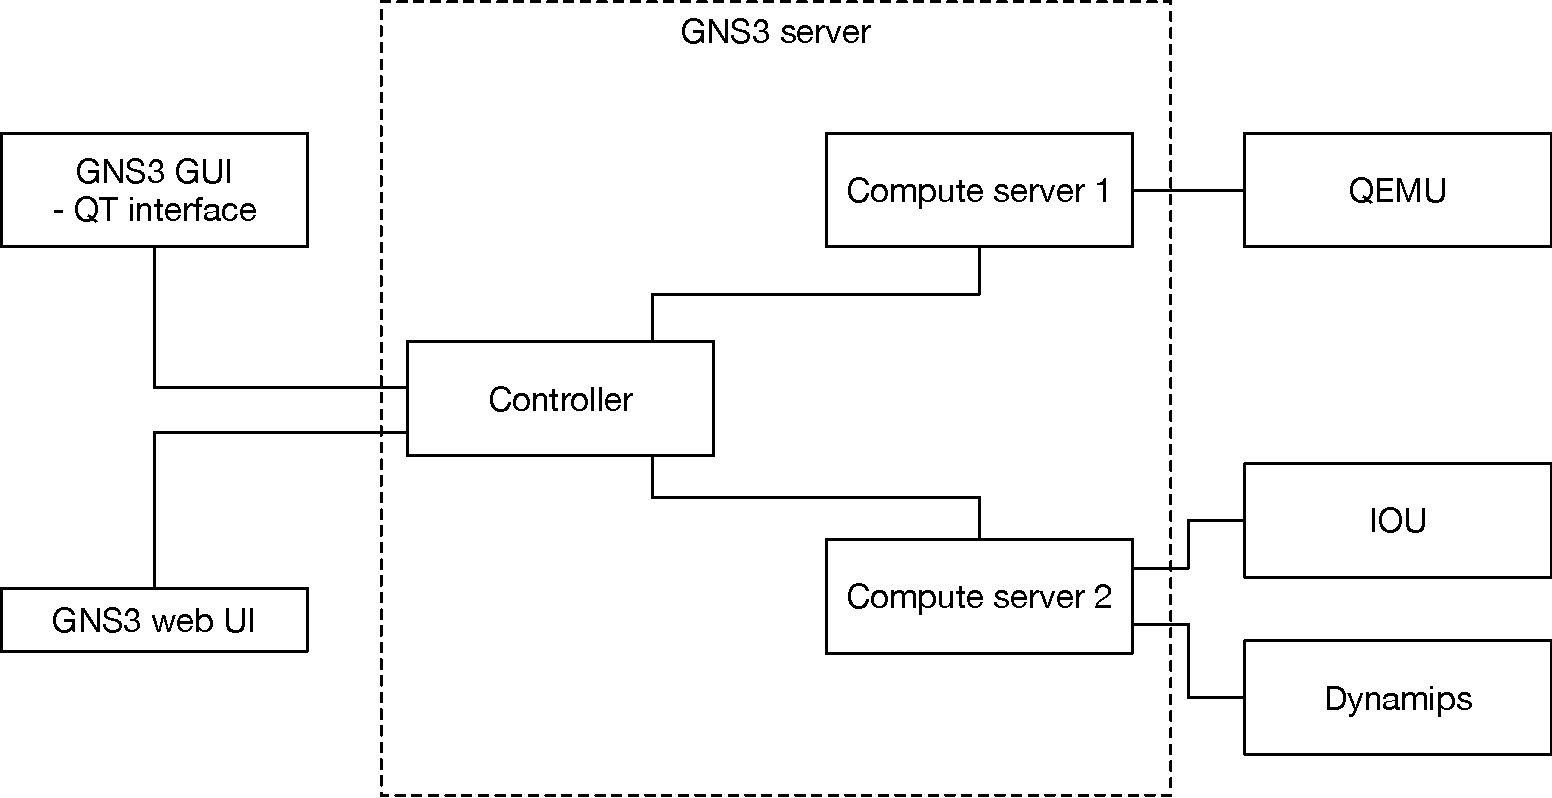
\includegraphics[width=0.8\textwidth]{gns3-docs-arch}
  \caption{The architecture of GNS3 (adapted from the official documentation)}
  \label{fig:gns3-docs-arch}
\end{figure}


\subsection{The simple client-server perspective}
\label{subsec:gns3clientserver}

GNS3 works, first and foremost, as a client-server application.
The standard installation for desktop provides all the necessary to components to fully(-ish) work on that physical machine, but the client doesn't have to be, and in many real scenarios isn't, running on the same host as the server.
However, in fact, a \textbf{topology}---the name GNS3 gives to its ``projects,'' which comprises of nodes (emulated/virtualized routers, switches, SDN-controllers, virtual PCs, interfaces for hardware network connections)---can be running in different machines, even on the ``backend'' side itself, as will be seen.

The \textbf{GNS3 server} exposes a public \acrshort{rest} \acrshort{api}, documented in~\cite{gns3devarch}, which is the way any client edits the opened topology or performs actions on the nodes contained therein, or in the GNS3 running environment.
GNS3 server, described more thoroughly afterwards, is the brains and central point of topology opened and in-execution.
It has first-hand knowledge of events that occur in the nodes, their status, their interfaces' status, and communicates with the several means existing to actually provide the \emph{emulation} for each specific node.
All of this will be analyzed and explained posteriorly.
For now, it suffices to see it as a central point, accessible by any number of clients, of a running topology.

To interact with the system, by editing a topology, or performing actions on nodes---all the items in the topology, which can be connected via links---, one or more users simultaneously can utilize a graphical client. The \textbf{GNS3 GUI}, part of a standard installation on any desktop operating system, namely macOS, a desktop Linux distribution (official repositories for Ubuntu exist), or Windows~\footnote{\url{https://gns3.com/software/download}}, is a cross-platform application developed using the Qt graphical toolkit~\cite{qttoolkit}.
They may also use a web UI (somewhat limited yet), or any tool, user-driven or automatic, programmed to send requests and receive responses according to the aforementioned REST specification.
The official clients, bundled with the GNS3 installation packages for desktop environments, GNS3 GUI and the official web UI, show an in-real-time view of the topology---e.g. the status of virtual network interfaces, or changes made by other client---thanks to WebSockets server-to-client calls~\cite{ytgns3arch22}. % TODO link WS to the glossary, when definition is available

% Figure fig:gns3-2hosts2routers-macOS
\begin{figure}
  \centering
  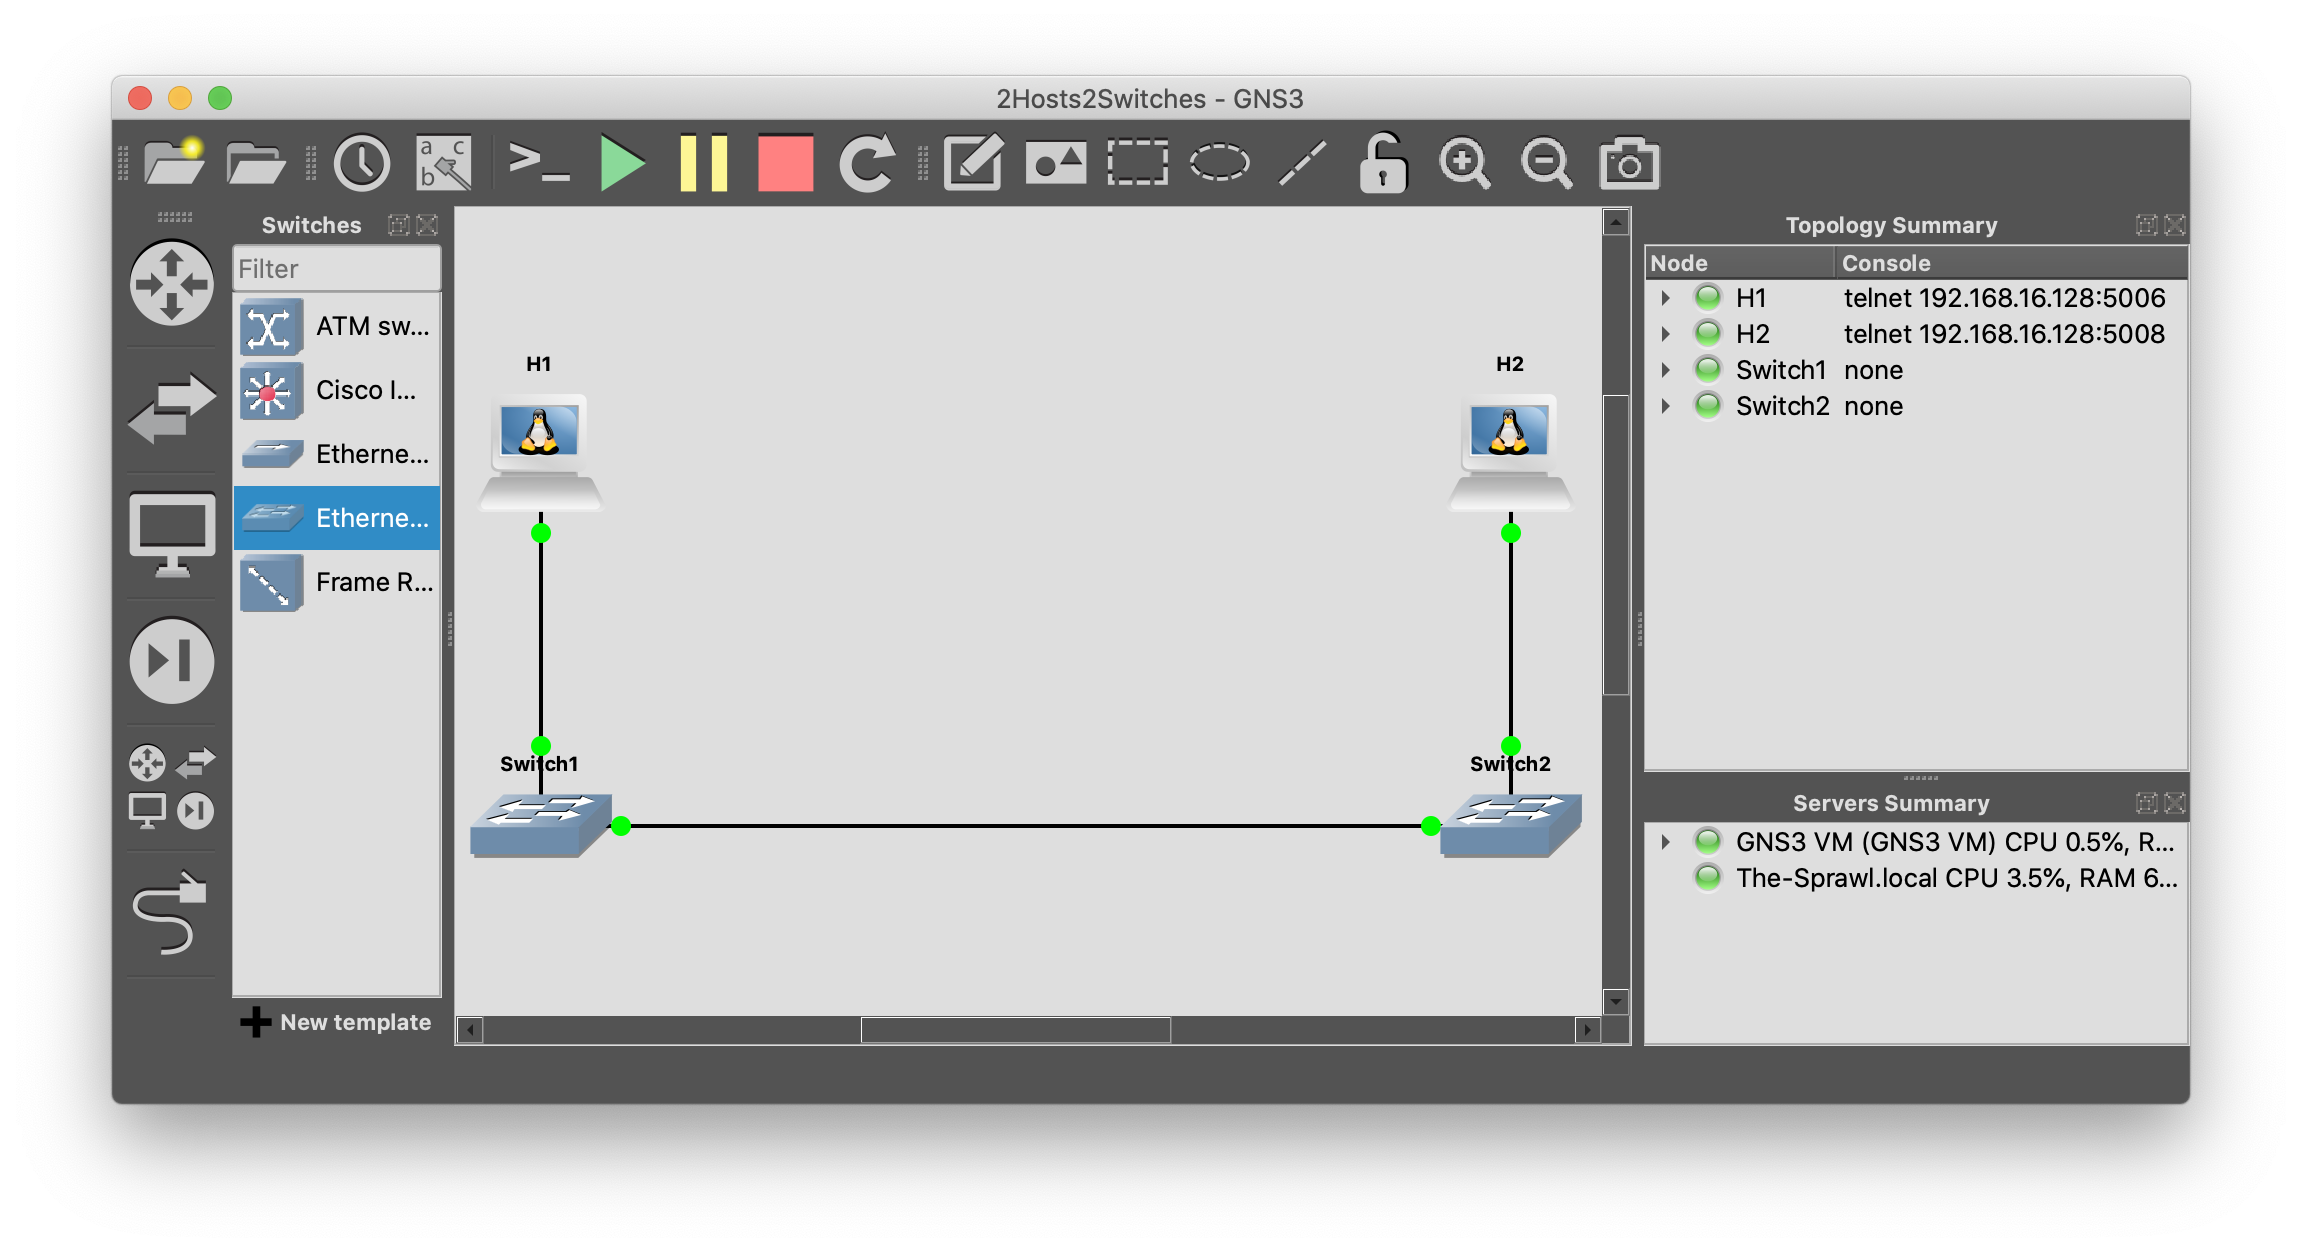
\includegraphics[width=0.8\textwidth]{gns3-2hosts2routers-macOS}
  \caption{Simple topology with only two switches and two virtual PCs as seen on the GUI in macOS}
  \label{fig:gns3-2hosts2routers-macOS}
\end{figure}


\subsection{The GNS3 server---distributed}
\label{subsec:gns3serverindetail}

The GNS3 server is a program with a code-base independent from other parts of the project.
The software package \texttt{gns3-server} can be obtained from official repositories for Linux systems to install it on servers without video interface, with users running some of the already mentioned clients in their laptops or desktop computers.
It is also possible to obtain a VMware ESXi image to directly spin-up a GNS3 server ready machine on an virtualized infrastructure.

The same program behaves as two different roles, both of which are necessary to get the GNS3 system working.

\begin{itemize}
	\item The \textbf{controller node}, or just ``controller,'' of which there can only be one instance per running topology, and is ``[its] decision point'' (Jeremy Grossmann's words); the process responsible by fulfilling the client's requests and postback real-time information to them and know the hosts where nodes may be running.
	\item The \textbf{compute node}, referred to simply as ``compute'' too, which, for one running topology, can be running $N$ times, one per each machine (physical or virtual) taking care of emulating one or more topology nodes (again: switches, routers, etc.).
	It is this separation and the ability to have multiple compute nodes that allows GNS3 to be configured in a way that can serve arbitrarily large topologies, since the cost in resources of an increasing number of ``live'' nodes can be balanced among an also increasing number of servers running a compute.
\end{itemize}

When the server is running on a single host, one \texttt{gns3-server} program instance (i.e. process) performs both roles, controller and compute.
However, when the server is distributed across one or more machines, communication between the controller and the computes on other hosts happens through a REST API.
That API is a private or internal one, unlike the one for client-server, and there isn't a programmer's manual for developing with it.
Only the (single) controller is supposed to communicate with each process acting as compute.

% end of section gns3architecture


% Section "Giving life to the topology-emulating nodes and links"
\section{Brining topologies to life---emulating nodes and links}
\label{sec:gns3emulating}

On section~\ref{sec:gns3architecture}, an overview of the way GNS3 is organized and runs in a distributed fashion was provided.
However, a crucial part is missing: how can the compute nodes, coordinated by the controller, which in turn is commanded by one or more clients, give life to the nodes that are put into a topology, seen in the GUI represented by their respective icons.
And also what mechanism is used to pass along the traffic transmited, received, switched, or any other action a possible node does while running via the links connected to the interfaces.

\subsection{Appliances}
\label{subsec:gns3appliances}

Each element of the set of possible nodes to be added to a topology on someone's GNS3 installation and setup is called an \textbf{appliance}.
GNS3 has a templating system for creating appliances, apart from the ones that come ``pre-installed.''
Many templates are immediately accessible from the GUI, and allow to prepare GNS3 to be able to put certain nodes on topology that it supports well but that cannot be distributed together with GNS3 for legal reasons or are simply too heavy and/or niche-oriented for bundling it by default to be worth it.
That is the case for commercial routers and switches that can be emulated in GNS3.

When, for example, a user intends to carry out one of the most common use-cases for GNS3---making a topology with Cisco IOSv nodes, which need Cisco's official disk images---that appliance is not ready to be used on the appliances dock on the GUI.
Instead they can easily access the template for it, which provides almost all inner parametrization and is a ``placeholder'' for that kind of node, provide the corresponding virtual disk image, which they should have downloaded and have licensed, and the client application takes care of uploading it to the server (local or remote), rendering the appliance available to be dragged-and-dropped into the topology canvas.

The panel (dubbed ``dock'' in GNS3 parlance) where the available devices are shown is depicted in figure~\ref{fig:gns3-appliances-dock}.
In this case, only the Cisco IOSvL2 switch and the Ubuntu Docker Guest were added after the base installation.
The other available nodes are stock.
Figure~\ref{fig:gns3-appliances-from-server-routers} shows the dialog where a partial list of available appliance templates is ready to be selected.

% Figures fig:gns3-appliances-dock and fig:gns3-appliances-from-server-routers
\begin{figure}
\centering
\begin{minipage}{.4\textwidth}
  \centering
  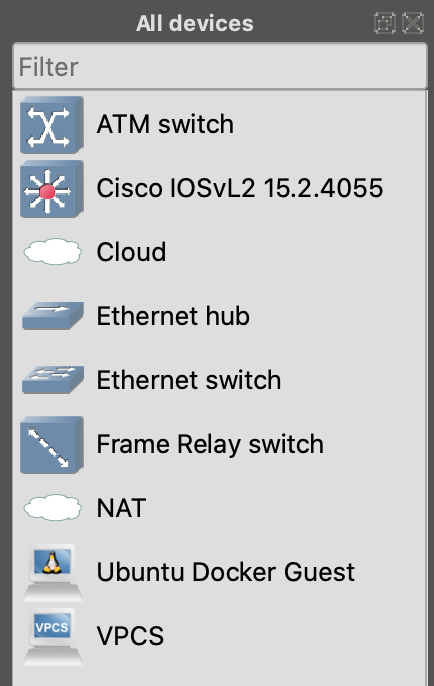
\includegraphics[width=.8\linewidth]{gns3-appliances-dock}
  \captionof{figure}{The appliances dock}
  \label{fig:gns3-appliances-dock}
\end{minipage}%
\begin{minipage}{.6\textwidth}
  \centering
  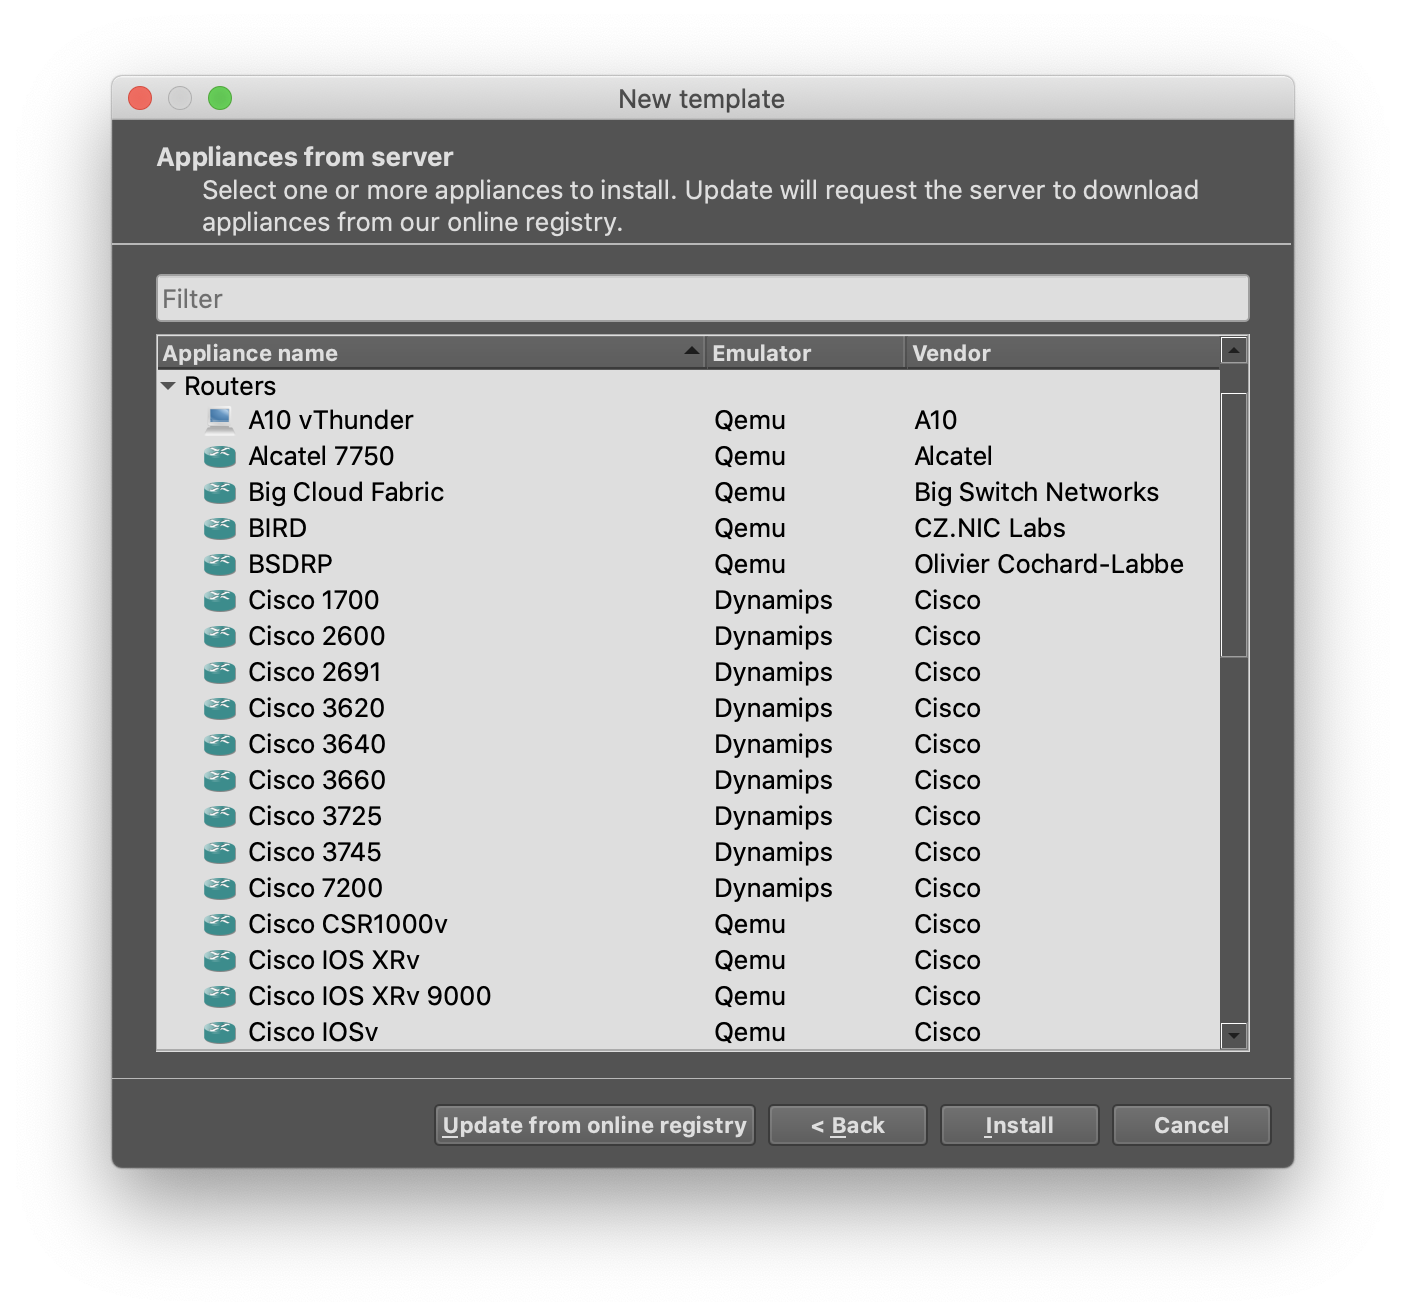
\includegraphics[width=.95\linewidth]{gns3-appliances-from-server-routers}
  \captionof{figure}{Some available router templates}
  \label{fig:gns3-appliances-from-server-routers}
\end{minipage}
\end{figure}


Deliberately, \emph{commercial} vendors of hardware, whose emulation is supported by GNS3, other than Cisco are excluded from this case-study for the following reasons:

\begin{enumerate}
  \item There isn't as near as many documentation and references in the literature, the web, or academic material for it as there is for Cisco.
  \item To narrow the scope of the investigation and this document, as the (again, commercial) network gear in laboratory used for the case study, FCT/NOVA's, is exclusively Cisco.
\end{enumerate}

Thus, this section is not intended to be exhaustive, or even less complete, in the sense of covering all the means GNS3 supplies out-of-the-box to emulate possible nodes in topologies.

\subsection{Dynamips and legacy Cisco routers}
\label{subsec:gns3dynamipslegacy}

GNS3 was initially built to leverage the Dynamips emulator~\cite{thebookofgns3}.
It consists of a pure hardware emulator for MIPS processors geared towards full-compatibility with a series of Cisco (now legacy) router hardware models, namely the 1700, 2600, 3600, 3700, and 7200 series. % TODO add 'MIPS' to gls
Not only it the emulator is able to execute MIPS machine-level instructions, it also is able to boot real, uncompressed images for the real hardware and provide virtual interfaces and slots for modules corresponding to those in the physical counterparts.

Dynamips does not support Cisco Catalyst layer-2 switches, only the aforementioned layer-3 modular routers.
All it offers for switching capabilities is, for some models, the ability to insert a module, called EtherSwitch, which provides 16 switched ports to the routers, and allows for \emph{some} experiments with the switching capabilities (VLANs, STP) to be made.
However, \cite{thebookofgns3}, which has a lengthy reference on using Dynamips, its advantages and disadvantages is clear in stating that it isn't without its limitations, which comprehensively listed in this reference.

In a video published in the already mentioned semi-official GNS3 YouTube channel, the software's creator Jeremy Grossmann clearly states that Dynamips is not recommended for production these days, since, as will be seen later, more modern and maintainable solutions exist. At the same time, the GNS3 creator and lead developer also states that there are not plans to remove Dynamips support in upcoming versions~\cite{ytdynamipsvpcs}.

That is not say that, if no ``advanced'' features are intended, Dynamips, whose processes are extremely light compared to most of the alternatives (cf. <REFER TO THE PERFORMANCE PART WHEN READY>), isn't the right solution, in the user or institution has access to licensed legacy IOS images. % TODO add ref to the performance part

\subsection{QEMU and Cisco IOSv}
\label{subsec:gns3ciscoiosv}

Another way to have Cisco gear inside a topology is using Cisco IOSv images, provided by the vendor itself as part of having access to their proprietary Virtual Internet Routing Lab (VIRL)~\cite{ciscovirl}.
IOSv, which concretely are IOSvL2 and IOSvL3 (standing for layer-2 and layer-3, respectively) are described as ``an implementation of Cisco IOS running as a full virtual machine on a hypervisor''~\cite{ciscoiosvinfo}.

On GNS3 this is accomplished via QEMU, a free and open source, general purpose emulator.
In particular, the way GNS3 uses QEMU is not as an emulator, but as a wrapper for KVM~\cite{whatiskvm}, which ensures extremely good virtualized performance, though naturally limited to the resources of the hypervisor machine~:
\begin{displayquote}
Run KVM and Xen virtual machines with near native performance\footnote{\url{https://www.qemu.org}}
\end{displayquote}

When an appliance for IOSv is added to a GNS3 setup using the template, a virtual disk image is provided and uploaded to the compute node.
It is then used for spinning up VMs with virtual interfaces running the operating system provided in the image. % TODO make this an acr statement

\subsection{Guests and other appliances}
\label{subsec:gns3guestsappliances}

``Guest''s is how GNS3 refers, on its interface, to hosts that can be added in topologies.
Here, host is meant in a conventional way, as what can be simply referred to as ``PCs'', ``servers'', or ``clients''.
GNS3 also supports other special end-devices, which are not explored in this thesis, such as the \acrshort{nat} or \emph{cloud} nodes.

A fresh install of GNS3 comes with only one guest appliance installed, VPCS.
This is a kind of simulated PC, developed by the GNS3 project\footnote{\url{https://github.com/GNS3/vpcs}} as a way to provide to GNS3's usable nodes, capable of transmitting and receiving network traffic through a virtual interface, via tools like \texttt{ping}.
Although the traffic it generates and receives is ``real'', and other nodes' interconnected to VPCS instances are not aware that it does not come from the usual applications on a host running a full-blown operating system, it doesn't have a kernel or possibility to run software over it.
A running VPCS node is simply a process that provides a virtual network interface and has a simple command-line interface to which the GNS3 user can \texttt{telnet}.

An advantage of these nodes is that they consume minimal resources, thus a topology can have a large quantity of them, and still allow to test topologies by checking connectivity on a variety of (potentially complex) scenarios.
They were especially useful on previous versions of GNS3, when the only way to have virtual hosts running full operating systems on GNS3 topologies---and, through it, test more advanced scenarios, using real-life software tools---, was to orchestrate heavy VirtualBox or VMware Workstation VMs, which are heavy, take time to boot, and its cost increases constantly with the number of instances.

Since version 2.1, though, GNS3 supports appliances based on Docker containers\footnote{Only on compute nodes running Linux}.
These are very lightweight and, excluding the resources consumed by the \texttt{dockerd} process (which runs only once on the host and still doesn't compare to one full-blown VM), each live container isn't noticeable heavier than a VPCS process, while still providing a real UNIX shell and possibility to run potentially potentially any GNU/Linux-compatible application.  % TODO confirmar (e citar)!!!
\begin{figure}
  \centering
  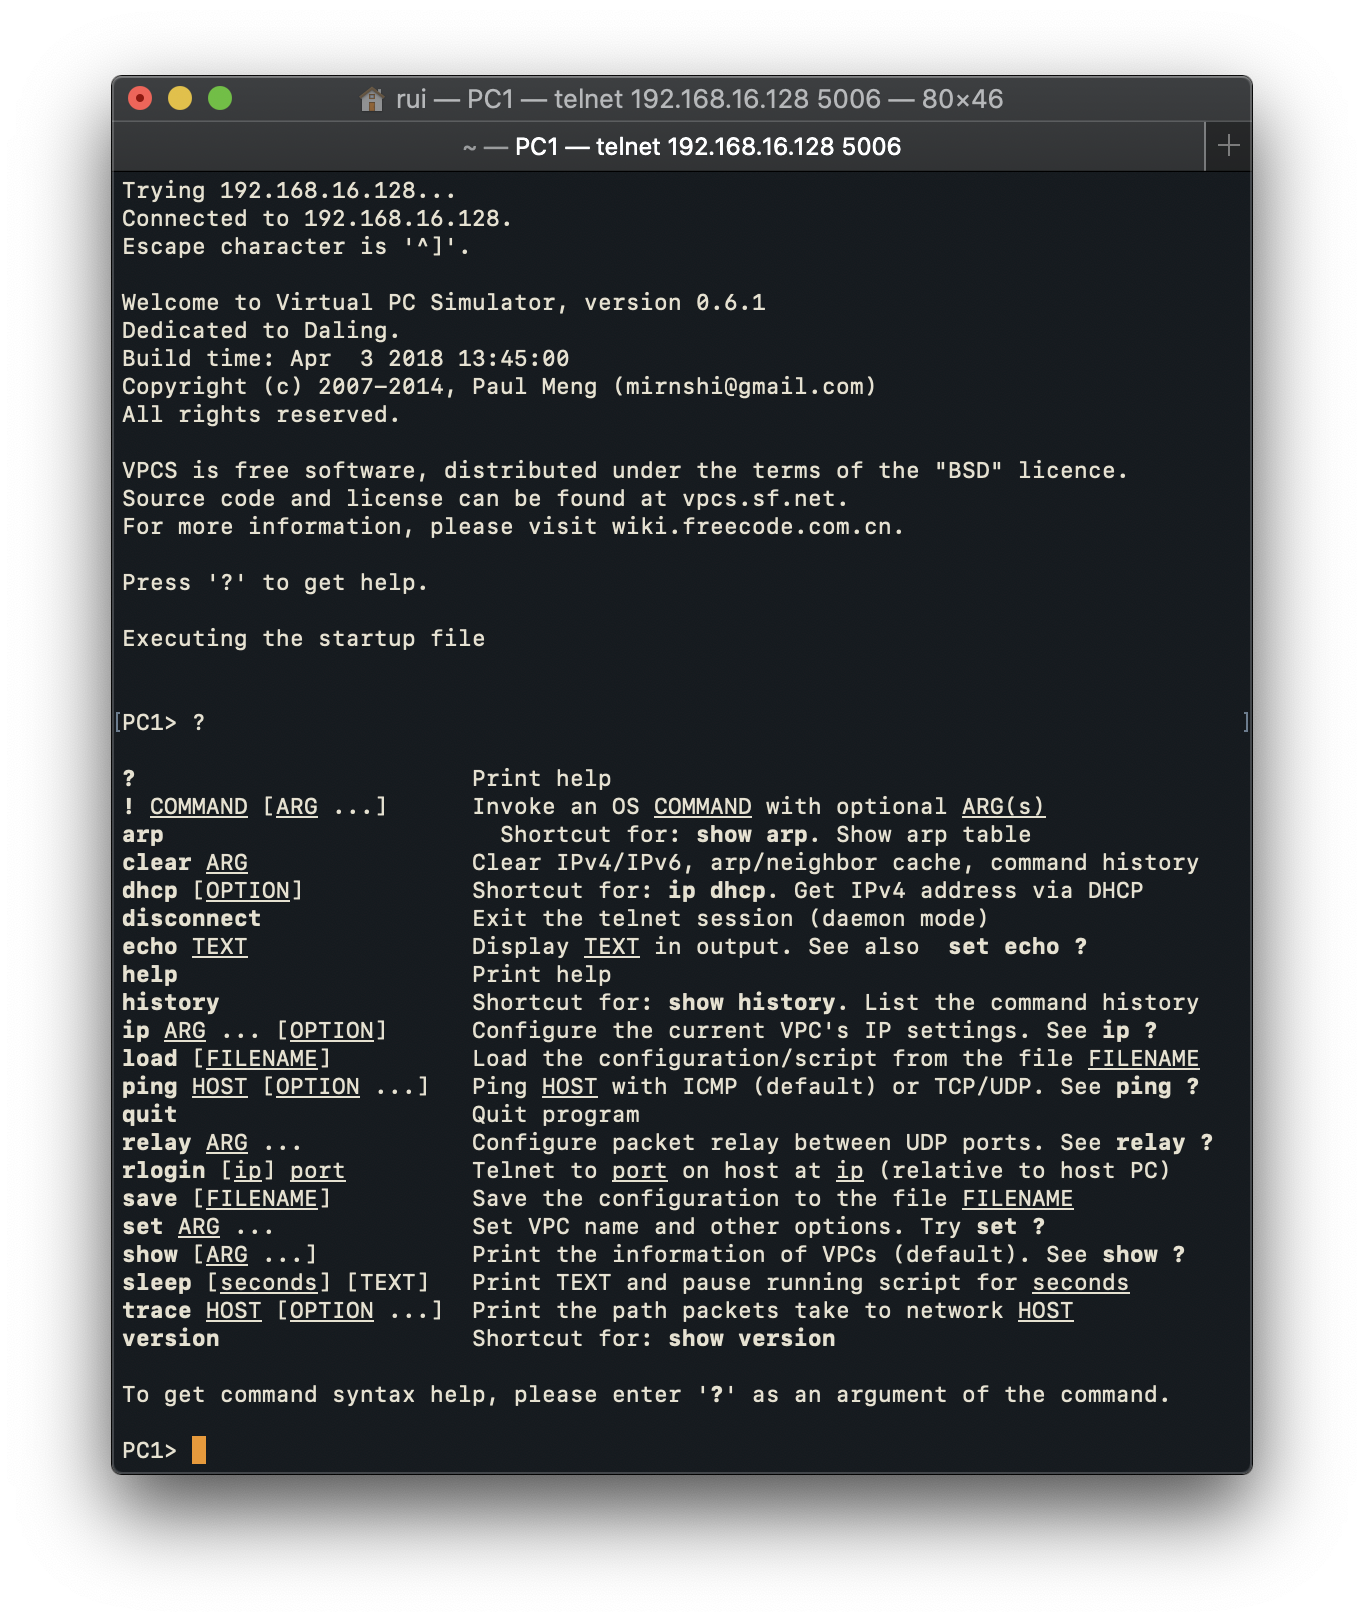
\includegraphics[width=0.6\textwidth]{gns3-vpcs-cli-help}
  \caption{A telnet session showing VPCS's list of commands}
  \label{fig:gns3-vpcs-cli-help}
\end{figure}

Due to this reason, the GNS3 project is recommending users to progressively stop using VPCS nodes and move towards Docker~\cite{ytdynamipsvpcs}.

The experiences carried out for this thesis use exclusively Docker containers as guests.

\subsection{Links}
\label{subsec:links}

A crucial part, and arguably the only element common to really \emph{any} GNS3 topology, is the emulation of data links.
For any two nodes to communicate, their \acrshortpl{nic} must be connected through a ``pipe,'' through which bits can flow in two directions.
GNS3 maintains a program, with an independent code base and which can be used independently, outside GNS3, called ubridge (in some places stylized as uBridge)\footnote{\url{https://github.com/GNS3/ubridge}}.
This program is the implementation of each of the straight lines that the user can draw on the canvas, clicking on two nodes, one after the other, and selecting the interfaces on each of them, to where the link is connected, reminding of a physical cable plugged on each free Ethernet port.

A deep study of ubridge wasn't carried out to know the implementation details.
What is practically observable is that, for each link, for each running interface on both of its ends (0, 1, or 2, depending on the status of the nodes), a user-level \texttt{ubridge} process exists on the compute's OS.

These processes listen on the virtual/software interface they were plugged in and encapsulate the traffic in UDP packages and send them through the compute's host OS network stack to the \texttt{ubridge} process on the other end of the logical link (it may or may not be running on the same compute). % TODO put UDP on glossary/acronyms
Conversely, they receive UDP datagrams, de-encapsulate the traffic inside them, and ``inject'' it back on the virtual interface they are attached to.

<IF TIME, INVESTIGATE AND BRIEFLY DESCRIBE HOW THIS ``ATTACHMENT'' WORKS> % TODO <- ver!

ubridge is known to provide functionality of configuring simulating packet loss (by frequency or percentage), time delay in packet delivery, corruption of a fraction of the packets, or a Berkeley Packet Filter (for filtering out packets matching an expression)~\cite{ubridgereadme}.

% end of section gns3emulating


% Section "Practical case study"
\section{Practical case study}
\label{sec:gns3practicalcasestudy}

Here will be described the process and results of the experiments carried out to assess aspects of the feasibility, and convenience, of using GNS3 in a real context of teaching and learning a computer networks subject in the University.
Hopefully, some of the gained insights can be extrapolated for other similar teaching facilities of slightly different characteristics.

To provide a real and well-defined set of examples to put in practice, the selected exercises and lab descriptions were taken out of the lab classes handouts for the 2018-2019 edition of ``Architecture and Protocols of Computer Networks,'' known by its Portuguese acronym APRC, an optional, graduate course offered at the Masters in Informatics at the FCT/NOVA.

\subsection{Overview of the considered labs and exercises}
\label{subsec:gns3consideredlabs}

Out of the 5 lab assignments, some of which span across more than one class, planned for a semester, only the first ones, which resort to the lab equipment to put in practice the subjects related to switching and layer-2 and ``legacy'' routing, as opposed to SDN, were considered. % TODO "span across?". Usar esta nota para pôr, se tiver ficado esquecido, referência no trabalho futuro aos exercícios de SDN que podem tirar partido de GNS3 e afins. SDN tem tem de estar nos acrónimos e glossário
Those are the exercises that, in the present, are expected to be done in the lab room, with real interconnected Cisco devices, issuing commands to the IOS command-line interface from the students' laptops.

The so-called ``lab-assignment1'' has a part to introduce the Cisco IOS and some basic commands for it.
Those are the ones to enter and escape the privileged mode, list the device's interfaces, and some other queries.
It also informs of how to load the running configuration of the device into the non-volatile memory, so that it persists after a shutdown, and how to do the opposite to discard unsaved running configurations and load the ones from the nonvolatile memory.

The second handout, ``lab-assignment2,'' is all about switching and layer-2 functionality.
It proposes a topology, expected to map the real interconnecting and physical disposition of devices in the room, of the nine switches, labels them with ``areas'' corresponding to cardinal points.
Students are then guided to answer questions about the expected behavior, e.g. in terms of reachability between hosts, according to parameters, which they should also issue in a coordinated fashion, for STP, VLANs, and trunks.

% Figures fig:gns3-aprc-lab2-handout-topology
\begin{figure}
  \centering
  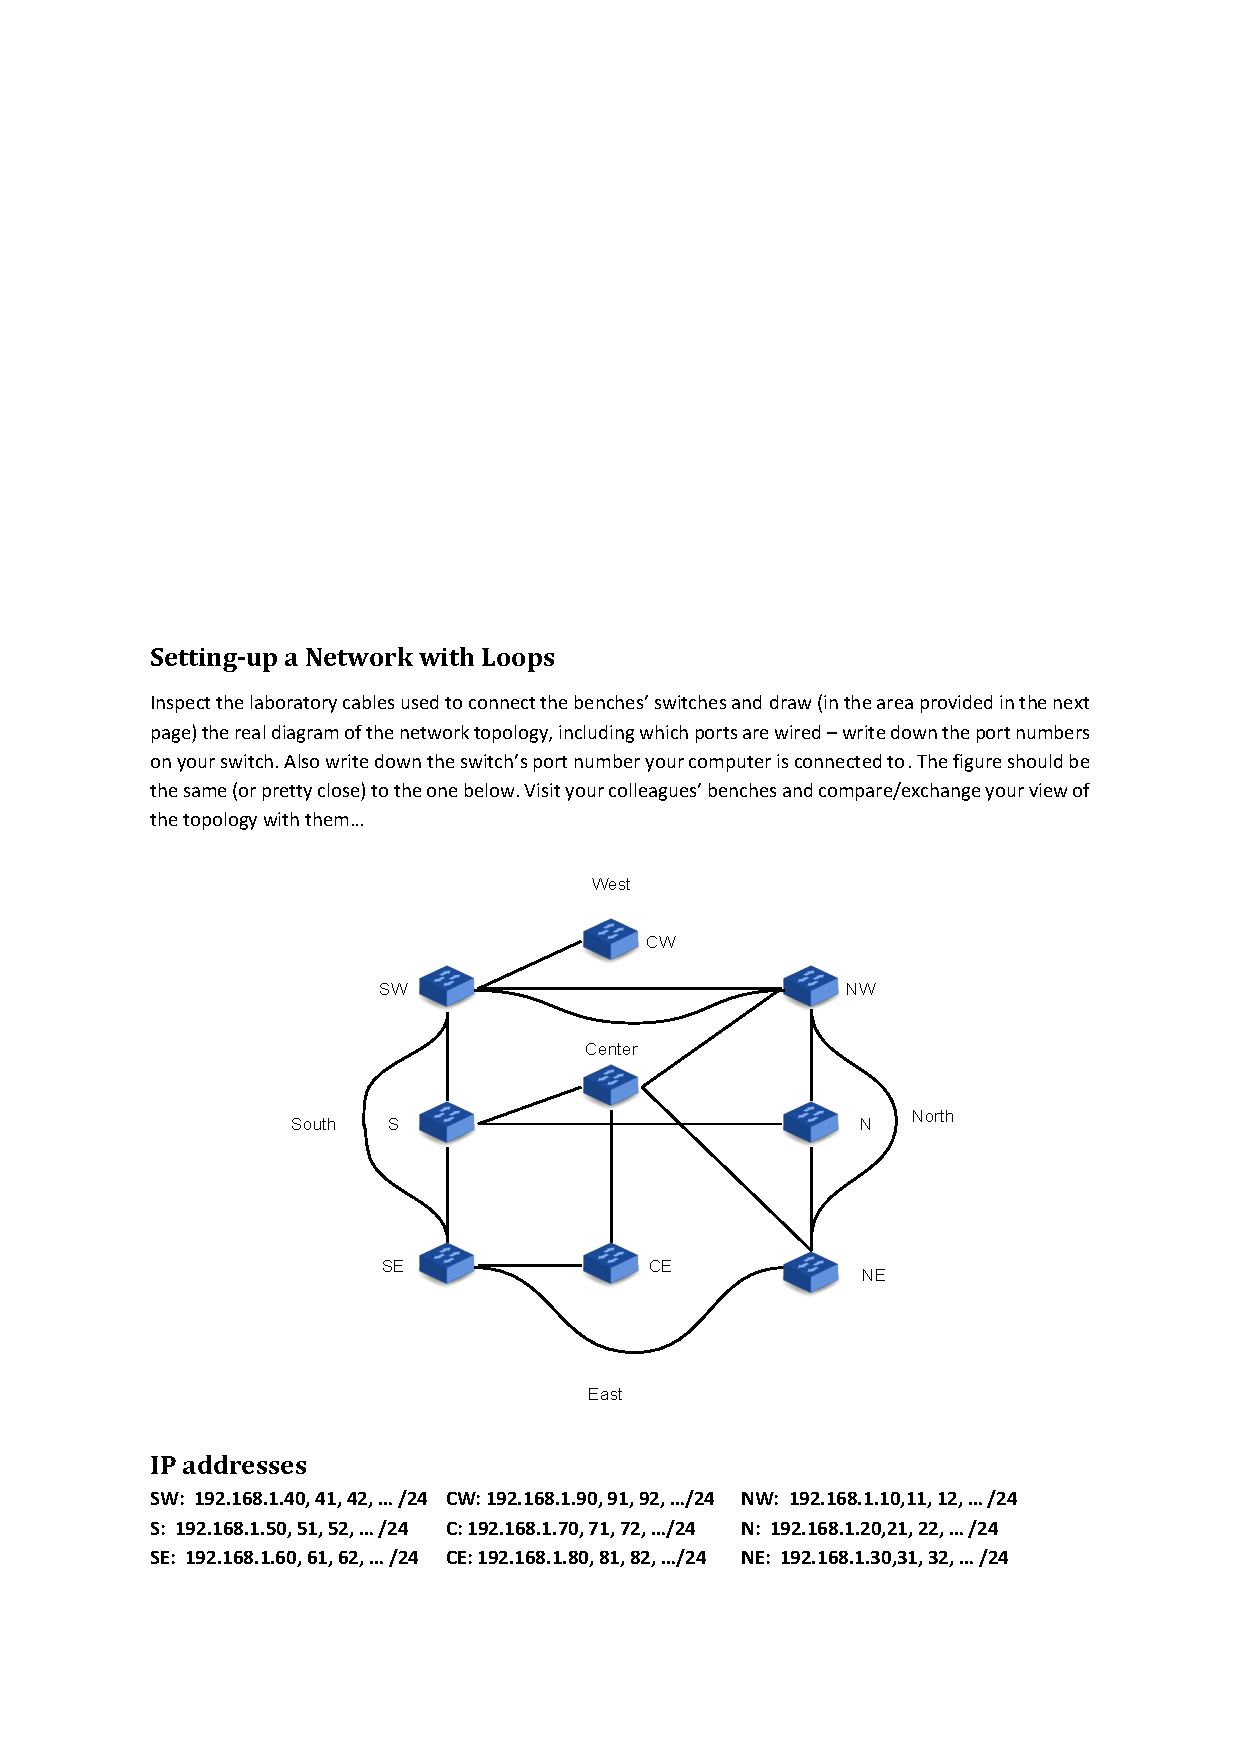
\includegraphics[width=0.8\textwidth, frame]{gns3-aprc-lab2-handout-topology}
  \caption{Section of ``lab-assignment2'' showing the topology}
  \label{fig:gns3-aprc-lab2-handout-topology}
\end{figure}


\subsection{Introduction to Cisco IOS and switching labs}
\label{subsec:gns3introswitching}

As said before, the first lab assignment introduces host-side commands (mostly Linux) and TCP/IP practical concepts such as IP address and \acrshort{mtu}, and its definition for the host's \acrfullpl{nic}.
The part of this lab handout that is to be performed on Cisco is perfectly doable on a GNS3 session with both (lighter) Dynamips EtherSwitch-enabled legacy routers or the more modern Cisco IOSvL2-3.
Double clicking on a node corresponding to one of these switches/routers, the GNS3 GUI will launch a terminal window on the user's desktop automatically executing the command necessary to create a \texttt{telnet} session to the node.

To perform the second lab, the topology described in figure~\ref{fig:gns3-aprc-lab2-handout-topology} (a section of the handout document) is physically implemented in the lab room with Cisco Catalyst switches interconnected accordingly with UTP-Ethernet cables supporting the data links.
The topology has loops which STP, running in the switches, is expected to eliminate by disabling certain link(s).
Part of the exercise is to foresee, according to the protocol's specification, which one(s) will be shutdown.

Execute this exercise in GNS3 already poses a bit of challenge, and introduces a dilemma.

Using the recommended IOSvL2 appliances on a typical laptop is not \emph{easy}.
First of all, IOSvL2, which as told before, runs on QEMU/KVM, is only supported on GNU/Linux computes.
On a laptop setup with macOS or Windows the standard GNS3 installation recommends having VMware Fusion or Workstation, respectively, installed and downloading the so-called GNS3 VM, which nothing else than a VM image, optimized for VMware's desktop hypervisors, containing a pre-made installation of the GNS3 server on an Ubuntu Server LTS.
The GNS3-gui for macOS and Windows then facilitates setting up the ``GNS3 VM'' to not need to setup a generic remote server to be used as compute, and is also able to open VMware Fusion or Workstation in the background and power on the GNS3 VM, so to serve as a standardized compute node.
Needless to say, this does not come without its overhead, both in terms of performance and practicality.

On the other hand, using a Dynamips EtherSwitch, that can be run on Dynamips directly on a macOS or Windows installation, and is much, much lighter, is not recommended anymore, since it requires legacy Cisco images, may not provide all the functionality, is reported to have bugs, etc.

In practice, though, if students have access to the IOS images compatible with the school's labs switches, all the exercises were proven to be performable on a laptop using Dynamips nodes.
VLANs are supported by these images, as well as STP, and standard routing protocols, such as OSPF (covered on a lab assignment too) are also run without problems on these equipments.

Summarizing, using Dynamips is no longer encouraged.
However, one assumes that the advice seen on the GNS3 forums, and on the videos and interviews with Jeremmy Grossmann already cited, for not using Dynamips is very much centered on advanced features and IOS interface compatibility.
However, in an undergraduate or graduate university level, where applying theoretical principles and seeing and doing in practice, in a controlled environment, not bound to any vendor tools, this advice may very well be irrelevant.

That said, Dynamips ensures actually better throughput on its EtherSwitch modules (surpassing the FastEthernet 100Mbps barrier) with a simple \texttt{iperf3} test between two hosts connected to the same device than an analogous scenario with IOSvL2 switches, as figure <INSERT SCREENSHOTS> shows.
It also is dramatically lighter on resource consumption, and users can emulate such nodes on their macOS or Windows---and obviously on GNU/Linux, which supports GNS3's emulation alternatives fully, too---without having any need for a distributed or load balanced architecture.

\subsection{Routing and OSPF on Cisco routers}
\label{subsec:gns3ospfrouting}

For the third lab assignment, divided into two parts, students are requested to connect their laptops to a topology similar to the one in the switching labs, but setting up the network interfaces on the nine multi-layer devices that interconnect them as layer-3 routing ports.
As written in the handout, the idea is that the routers interconnect the backbone of the offices of a nation-wide corporation.
Therefore, the computers in each bench (office), have its interface in different IP prefixes, corresponding to separate LANs. % TODO add gls reference

First, to set up set routing, students are requested to design an addressing plan, setting up prefixes and hosts on the routing interfaces connected each router to another, and then setup manually, using IOS's interface, static routes that allow to connect each office's LAN to another.
After this, students can configure the router/switch virtual interface (which is also configured to be on its respective LAN) as the default gateway and \texttt{ping} each other's computer.

The second goal is to, instead of doing the routing statically, configure the routers to use OSPF, and perform a set of analysis and variations on the exercise, such as changing the bandwidth of some links, turning other links off and foreseeing the behavior according to the specification of the protocol.

Students can also use Wireshark to capture the data OSPF exchanges across the network.

Although the considerations related to using Dynamips versus using IOSv are also applicable here, the complexity of this exercise will be used to demonstrate two facets of GNS3's functionality and setup-wise flexibility, namely:
\begin{itemize}
  \item Distributing the load between many servers (computes)---useful to scale, and particularly necessary when emulating heavier nodes such as IOSv instances.
  \item Topology snapshots
\end{itemize}

\subsubsection{Running more than one server. Load balancing}

The importance of load balancing is obvious in general. GNS3's topologies are JSON files describing which devices exist on it, their names, meta-information to be used in the moment where each emulator is executed, and which links connect which virtual interfaces~\cite{thebookofgns3}.
Therefore, there is not a practical limitation of the central points, the controller and the GUI, in the size which a topology can have.
It is possible, and examples across the web are given, of enormous topologies.

The way this is possible is by using separate hosts to run an instance of the GNS3-server, in the role of a compute, receiving instructions from the controller (in turn controlled by the user using, for instance, the GNS3 GUI) to interact with the running emulators.
As long as the total amount of emulators and ubridge processe attached to those processes running on each of those hosts doesn't use too many resources of each compute-host, there isn't exactly any bottle-neck, since the emulated nodes execute independently of GNS3's ``brains''.

Unless the user is editing the topology, creating or deleting nodes and links, starting and stopping machines, or other orchestration-specific tasks, the interaction with the running nodes is done thought direct \texttt{telnet} connections to the emulator processes from terminal windows accessible to the user, outside of GNS3.
To make that easier, if using the GNS3 GUI, a user can double click on e.g. a ``powered-on'' switched or Ubuntu Docker Guest, and a helper is transparently executed which will open a terminal window on that (graphical) host, automatically running a command like \texttt{telnet 10.170.138.106 5001}---where \texttt{10.170.138.106} is the IP address of the compute host where a certain node is running and \texttt{5001} is the concrete TCP port where the emulator process is listening to accept connections to the console.

In the case of the lab assignment 3 (layer-3 routing and OSPF), two servers were setup on the FCT/NOVA DI infrastructure.
One was running the GNS3 server as the controller (and also as compute for some nodes), and the other only as a ``secondary'' compute node.
Note that there is no reason to assume that the ``primary'' (generally, the controller) is the host with the most resources.
In fact, this wasn't the case in the architecture set up for this experiment.

% end of section gns3practicalcasestudy


% Section "Performance and resources considerations"
\section{Performance and resources considerations}
\label{sec:gns3performance}

% end of section gns3performance


% end of chapter
